\section{Bestemmelse af vandtemperatur i rør}
Produktet skal kunne overvåge vandspildet uden at have regulerbare funktioner. Det skal kunne måle temperaturen i henholdvis rummet og  overfladen på vandrøret, endvidere skal det kunne sammenligne de to temperature. \fxnote{for at måle fugtigheden}.
Graf \ref{vandspild_graf_normal} viser et eksempel på hvordan temperaturændringerne forekommer, hvis det antages at vandspildet negliseres og temperaturen på røret derfor er lig med temperaturen i rummet.  
\\
\\
\begin{figure}[h!]
  \centering
  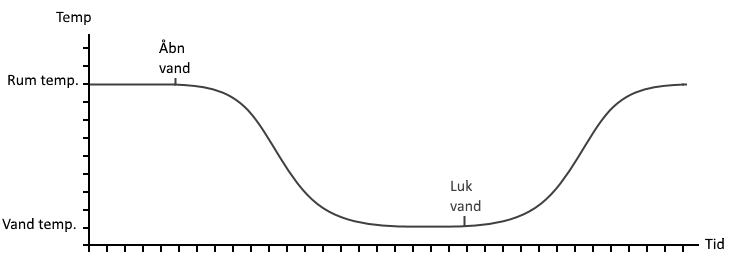
\includegraphics[width=0.7\textwidth]{figures/vandspild_graf_normal.png}
  \caption{Grafen viser overvågningssystemet uden vand spild.}
  \label{vandspild_graf_normal}
\end{figure}
\fxnote{ret figur, ingen grund til den er så høj når vi kun har 2 punkter på x aksen}
\\
\\
Tilførelsen af nyt vand til huset ændre rørets temperatur og derfor vil der forekomme temperatursvingninger, som målingen viser vandspildet ud fra. Nedernstående graf \ref{vandspild_graf_spild} viser et eksempel på temperaturændringer ved vandspild på et rør.
\\
\\
\begin{figure}[h!]
  \centering
  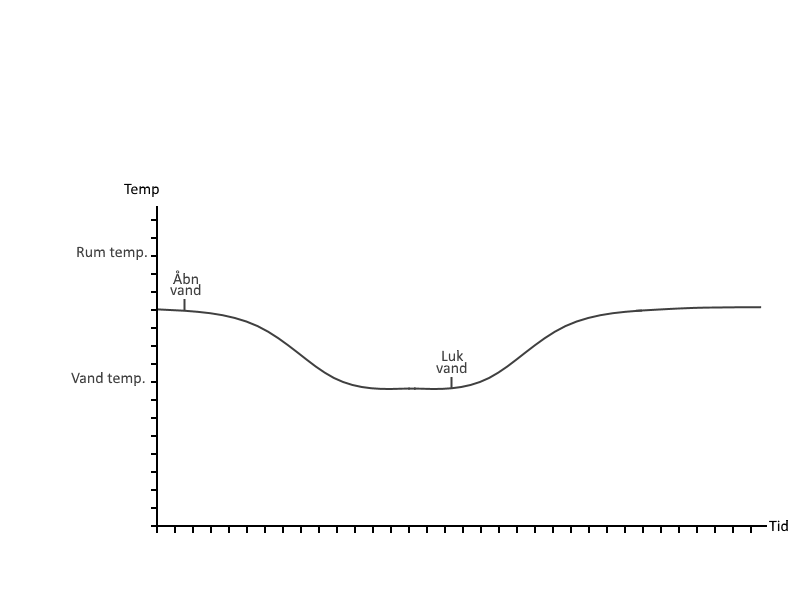
\includegraphics[width=0.7\textwidth]{figures/vandspild_graf_spild.png}
  \caption{Grafen viser overvågningssystemet med vandspild.}
  \label{vandspild_graf_spild}
\end{figure}
\fxnote{ret figur, ingen grund til den er så høj når vi kun har 2 punkter på x aksen}
\\
\\
Her ses hvordan hviletemperaturen på røret aldrig når temperaturen i rummet, da vandet aldrig ligger helt stille og derfor tilfører en konstant koldere temperatur.    